\documentclass{standalone}
\usepackage{tikz}
\usepackage{ctex,siunitx}
\setCJKmainfont{Noto Serif CJK SC}
\usepackage{tkz-euclide}
\usepackage{amsmath}
\usetikzlibrary{patterns, calc,3d}
\usetikzlibrary {decorations.pathmorphing,decorations.pathreplacing,decorations.shapes}
\begin{document}
\small
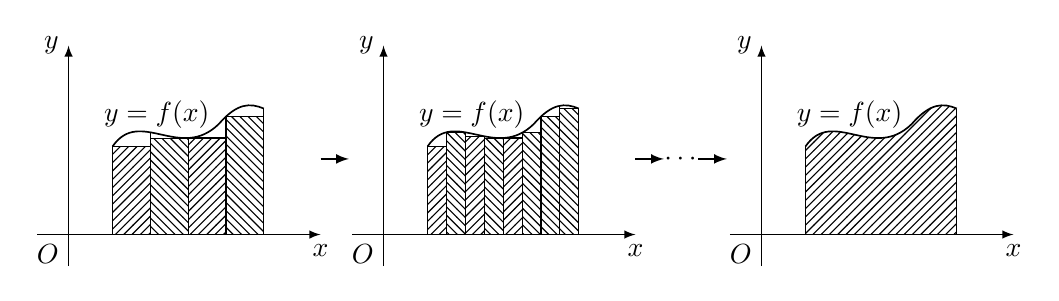
\begin{tikzpicture}[>=latex,scale=0.8]
  \begin{scope}
    \draw[->](-0.5,0)--(4,0)node[below]{$x$};
    \draw[->](0,-0.5)--(0,3)node[left]{$y$};
    \node at (0,0)[below left]{$O$};
    \draw[semithick](0.700,1.400)..controls(1.130,2.023)and(1.771,1.156)..
    (2.385,1.754)..controls(2.677,2.090)and(2.881,2.092)..(3.100,2.000);
    \draw(0.7,1.4)--(0.7,0)(3.1,2)--(3.1,0);
    \draw[pattern=north east lines](0.7,0)rectangle++(0.6,1.4);
    \draw[pattern=north west lines](1.3,0)rectangle++(0.6,1.531);
    \draw[pattern=north east lines](1.9,0)rectangle++(0.6,1.532);
    \draw[pattern=north west lines](2.5,0)rectangle++(0.6,1.873);
    \draw[densely dashed](1.3,0)--(1.3,1.6217);
    \draw[densely dashed](1.9,0)--(1.9,1.5324);
    \draw[densely dashed](2.5,0)--(2.5,1.8732);
    \node at (1.4,1.9){$y=f(x)$};
  \end{scope}
  \begin{scope}[xshift=5cm]
    \draw[->](-0.5,0)--(4,0)node[below]{$x$};
    \draw[->](0,-0.5)--(0,3)node[left]{$y$};
    \node at (0,0)[below left]{$O$};
    \draw[semithick](0.700,1.400)..controls(1.130,2.023)and(1.771,1.156)..
    (2.385,1.754)..controls(2.677,2.090)and(2.881,2.092)..(3.100,2.000);
    \draw(0.7,1.4)--(0.7,0)(3.1,2)--(3.1,0);
    \draw[pattern=north east lines](0.7,0)rectangle++(0.3,1.4);
    \draw[pattern=north west lines](1.0,0)rectangle++(0.3,1.6217);
    \draw[pattern=north east lines](1.3,0)rectangle++(0.3,1.5596);
    \draw[pattern=north west lines](1.6,0)rectangle++(0.3,1.5311);
    \draw[pattern=north east lines](1.9,0)rectangle++(0.3,1.5324);
    \draw[pattern=north west lines](2.2,0)rectangle++(0.3,1.6152);
    \draw[pattern=north west lines](2.5,0)rectangle++(0.3,1.8732);
    \draw[pattern=north west lines](2.8,0)rectangle++(0.3,2);
    \draw[densely dashed](1.3,0)--(1.3,1.6217);
    \draw[densely dashed](1.9,0)--(1.9,1.5324);
    \draw[densely dashed](2.5,0)--(2.5,1.8732);
    \draw[densely dashed](2.8,0)--(2.8,2.0444);
    \node at (1.4,1.9){$y=f(x)$};
  \end{scope}
  \begin{scope}[xshift=11cm]
    \draw[->](-0.5,0)--(4,0)node[below]{$x$};
    \draw[->](0,-0.5)--(0,3)node[left]{$y$};
    \node at (0,0)[below left]{$O$};
    \draw[semithick](0.700,1.400)..controls(1.130,2.023)and(1.771,1.156)..
    (2.385,1.754)..controls(2.677,2.090)and(2.881,2.092)..(3.100,2.000);
    \fill[pattern=north east lines](0.700,0)--(0.700,1.400)..controls(1.130,2.023)and(1.771,1.156)..
    (2.385,1.754)..controls(2.677,2.090)and(2.881,2.092)..(3.100,2.000)--(3.1,0);
    \draw(0.7,1.4)--(0.7,0)(3.1,2)--(3.1,0);
    \node at (1.4,1.9){$y=f(x)$};
  \end{scope}
  
  \foreach \x in {4,9,10}{\draw[semithick,->](\x,1.2)--++(0.45,0);}
  \node at (9.75,1.2){$\cdots$};
\end{tikzpicture}
\end{document}